%package list
\documentclass{article}
\usepackage[top=3cm, bottom=3cm, outer=3cm, inner=3cm]{geometry}
\usepackage{multicol}
\usepackage{graphicx}
\usepackage{url}
%\usepackage{cite}
\usepackage{hyperref}
\usepackage{array}
%\usepackage{multicol}
\newcolumntype{x}[1]{>{\centering\arraybackslash\hspace{0pt}}p{#1}}
\usepackage{natbib}
\usepackage{pdfpages}
\usepackage{multirow}
\usepackage[normalem]{ulem}
\useunder{\uline}{\ul}{}
\usepackage{svg}
\usepackage{xcolor}
\usepackage{listings}
\lstdefinestyle{ascii-tree}{
    literate={├}{|}1 {─}{--}1 {└}{+}1 
  }
\lstset{basicstyle=\ttfamily,
  showstringspaces=false,
  commentstyle=\color{red},
  keywordstyle=\color{blue}
}
%\usepackage{booktabs}
\usepackage[labelformat=empty]{caption}
\usepackage{subcaption}
\usepackage{float}
\usepackage{array}

\newcolumntype{M}[1]{>{\centering\arraybackslash}m{#1}}
\newcolumntype{N}{@{}m{0pt}@{}}


%%%%%%%%%%%%%%%%%%%%%%%%%%%%%%%%%%%%%%%%%%%%%%%%%%%%%%%%%%%%%%%%%%%%%%%%%%%%
%%%%%%%%%%%%%%%%%%%%%%%%%%%%%%%%%%%%%%%%%%%%%%%%%%%%%%%%%%%%%%%%%%%%%%%%%%%%
\newcommand{\itemEmail}{cmestasz@unsa.edu.pe}
\newcommand{\itemStudent}{Christian Mestas Zegarra}
\newcommand{\itemCourse}{Fundamentos de la Programación 2}
\newcommand{\itemCourseCode}{1701213}
\newcommand{\itemSemester}{II}
\newcommand{\itemUniversity}{Universidad Nacional de San Agustín de Arequipa}
\newcommand{\itemFaculty}{Facultad de Ingeniería de Producción y Servicios}
\newcommand{\itemDepartment}{Departamento Académico de Ingeniería de Sistemas e Informática}
\newcommand{\itemSchool}{Escuela Profesional de Ingeniería de Sistemas}
\newcommand{\itemAcademic}{2023 - B}
\newcommand{\itemInput}{Del 06 Diciembre 2023}
\newcommand{\itemOutput}{Al 11 Diciembre 2023}
\newcommand{\itemPracticeNumber}{12}
\newcommand{\itemTheme}{Clase Soldado - Menú}
%%%%%%%%%%%%%%%%%%%%%%%%%%%%%%%%%%%%%%%%%%%%%%%%%%%%%%%%%%%%%%%%%%%%%%%%%%%%
%%%%%%%%%%%%%%%%%%%%%%%%%%%%%%%%%%%%%%%%%%%%%%%%%%%%%%%%%%%%%%%%%%%%%%%%%%%%

\usepackage[english,spanish]{babel}
\usepackage[utf8]{inputenc}
\AtBeginDocument{\selectlanguage{spanish}}
\renewcommand{\figurename}{Figura}
\renewcommand{\refname}{Referencias}
\renewcommand{\tablename}{Tabla} %esto no funciona cuando se usa babel
\AtBeginDocument{%
	\renewcommand\tablename{Tabla}
}

\usepackage{fancyhdr}
\pagestyle{fancy}
\fancyhf{}
\setlength{\headheight}{30pt}
\renewcommand{\headrulewidth}{1pt}
\renewcommand{\footrulewidth}{1pt}
\fancyhead[L]{\raisebox{-0.2\height}{
\includegraphics[width=3cm]{img/logo_episunsa.png}}}
\fancyhead[C]{\fontsize{7}{7}\selectfont	\itemUniversity \\ \itemFaculty \\ \itemDepartment \\ \itemSchool \\ \textbf{\itemCourse}}
\fancyhead[R]{\raisebox{-0.2\height}{
\includegraphics[width=1.2cm]{img/logo_abet}}}
\fancyfoot[L]{Christian Mestas}
\fancyfoot[C]{\itemCourse}
\fancyfoot[R]{Página \thepage}

% para el codigo fuente
\usepackage{listings}
\usepackage{color, colortbl}
\definecolor{dkgreen}{rgb}{0,0.6,0}
\definecolor{gray}{rgb}{0.5,0.5,0.5}
\definecolor{mauve}{rgb}{0.58,0,0.82}
\definecolor{codebackground}{rgb}{0.95, 0.95, 0.92}
\definecolor{tablebackground}{rgb}{0.8, 0, 0}

\lstset{frame=tb,
	language=bash,
	aboveskip=3mm,
	belowskip=3mm,
	showstringspaces=false,
	columns=flexible,
	basicstyle={\small\ttfamily},
	numbers=none,
	numberstyle=\tiny\color{gray},
	keywordstyle=\color{blue},
	commentstyle=\color{dkgreen},
	stringstyle=\color{mauve},
	breaklines=true,
	breakatwhitespace=true,
	tabsize=3,
	backgroundcolor= \color{codebackground},
}

\begin{document}

\vspace*{10px}

\begin{center}
	\fontsize{17}{17} \textbf{ Informe de Laboratorio \itemPracticeNumber}
\end{center}
\centerline{\textbf{\Large Tema: \itemTheme}}
%\vspace*{0.5cm}	

\begin{flushright}
	\begin{tabular}{|M{2.5cm}|N|}
		\hline
		\rowcolor{tablebackground}
		\color{white} \textbf{Nota} \\
		\hline
		\\[30pt]
		\hline
	\end{tabular}
\end{flushright}

\begin{table}[H]
	\begin{tabular}{|M{4.7cm}|M{4.8cm}|M{4.8cm}|}
		\hline
		\rowcolor{tablebackground}
		\color{white} \textbf{Estudiante} & \color{white}\textbf{Escuela} & \color{white}\textbf{Asignatura}                                        \\
		\hline
		{\itemStudent \par \itemEmail}    & \itemSchool                   & {\itemCourse \par Semestre: \itemSemester \par Código: \itemCourseCode} \\
		\hline
	\end{tabular}
\end{table}

\begin{table}[H]
	\begin{tabular}{|M{4.7cm}|M{4.8cm}|M{4.8cm}|}
		\hline
		\rowcolor{tablebackground}
		\color{white}\textbf{Laboratorio} & \color{white}\textbf{Tema} & \color{white}\textbf{Duración} \\
		\hline
		\itemPracticeNumber               & \itemTheme                 & 04 horas                       \\
		\hline
	\end{tabular}
\end{table}

\begin{table}[H]
	\begin{tabular}{|M{4.7cm}|M{4.8cm}|M{4.8cm}|}
		\hline
		\rowcolor{tablebackground}
		\color{white}\textbf{Semestre académico} & \color{white}\textbf{Fecha de inicio} & \color{white}\textbf{Fecha de entrega} \\
		\hline
		\itemAcademic                            & \itemInput                            & \itemOutput                            \\
		\hline
	\end{tabular}
\end{table}

%%%%%%%%%%%%%%%%%%%%%%%%%%%%%%%%%%%%%%%%%%%%%%%%%%%%%%%%%%%%%%%%%%%%%%
\section{Tarea}
\begin{itemize}
	\item \textbf{Item 1:} Puede reutilizar todo el código del laboratorio 11, pero ahora el objetivo es
	      gestionar los ejércitos autogenerados.
	\item \textbf{Item 2:} Al ejecutar el videojuego, el programa deberá dar las opciones:\\
	      1. Juego rápido (tal cual como en el laboratorio 11)
	      Al acabar el juego mostrar las opciones de volver a jugar y de volver al
	      menú principal. También se deberá tener la posibilidad de cancelar el
	      juego actual en cualquier momento, permitiendo escoger entre empezar
	      un juego totalmente nuevo o salir al menú principal.\\
	      2. Juego personalizado: permite gestionar ejércitos. Primero se generan
	      los 2 ejércitos con sus respectivos soldados y se muestran sus datos
	      Luego se tendrá que escoger cuál de los 2 ejércitos se va a gestionar,
	      después se mostrarán las siguientes opciones:\\
	      1) Crear Soldado: permitirá crear un nuevo soldado personalizado
	      y añadir al final del ejército (recordar que límite es de 10
	      soldados por ejército)\\
	      2) Eliminar Soldado (no debe permitir un ejército vacío)\\
	      3) Clonar Soldado (crea una copia exacta del soldado) y se añade
	      al final del ejército (recordar que límite es de 10 soldados por
	      ejército)\\
	      4) Modificar Soldado (con submenú para cambiar alguno de los
	      atributos nivelAtaque, nivelDefensa, vidaActual)\\
	      5) Comparar Soldados (verifica si atributos: nombre, nivelAtaque,
	      nivelDefensa, vidaActual y vive son iguales)\\
	      6) Intercambiar Soldados (intercambia 2 soldados en sus posiciones
	      en la estructura de datos del ejército)\\
	      7) Ver soldado (Búsqueda por nombre)\\
	      8) Ver ejército\\
	      9) Sumar niveles (usando Method-Call Chaining), calcular las
	      sumatorias de nivelVida, nivelAtaque, nivelDefensa, velocidad de
	      todos los soldados de un ejército
	      1. Por ejemplo, si ejército tendría 3 soldados:
	      2. s=s1.sumar(s2).sumar(s3);
	      3. s es un objeto Soldado nuevo que contendría las
	      sumatorias de los 4 atributos indicados de los 3 soldados.
	      Ningún soldado cambia sus valores\\
	      10) Jugar (se empezará el juego con los cambios realizados) y con
	      las mismas opciones de la opción 1 del menú principal.\\
	      11) Volver (muestra el menú principal)
	      Después de escoger alguna de las opciones 1) a 9) se podrá volver a
	      elegir uno de los ejércitos y se mostrarán las opciones 1) a 11)\\
	      3. Salir
\end{itemize}
%%%%%%%%%%%%%%%%%%%%%%%%%%%%%%%%%%%%%%%%%%%%%%%%%%%%%%%%%%%%%%%%%%%%%%
\pagebreak

\section{Equipos, materiales y temas utilizados}
\begin{itemize}
	\item Sistema Operativo Microsoft Windows 10 Pro 64 bits
	\item Visual Studio Code 1.82.2
	\item Java Development Kit 17.0.1
	\item Git 2.41.0.windows.1
	\item Windows PowerShell 5.1.19041.3031
	\item Cuenta en GitHub con el correo institucional.
	      %%%%%%%%%%%%%%%%%%%%%%%%%%%%%%%%%%%%%%%%%%%%%%%%%%%%%%%%%%%%%%%%%%%%%%
	\item Programación Orientada a Objetos
	\item HashMap de Objetos
	\item ArrayList de Objetos
	\item Ordenamientos burbuja y por selección.
	      %%%%%%%%%%%%%%%%%%%%%%%%%%%%%%%%%%%%%%%%%%%%%%%%%%%%%%%%%%%%%%%%%%%%%%
\end{itemize}

\section{URL de Repositorio Github}
\begin{itemize}
	\item URL del Repositorio GitHub para clonar o recuperar.
	\item \url{https://github.com/cmestasz/fp2-23b.git}
	      %%%%%%%%%%%%%%%%%%%%%%%%%%%%%%%%%%%%%%%%%%%%%%%%%%%%%%%%%%%%%%%%%%%%%%
	\item URL para el laboratorio 12 en el Repositorio GitHub.
	\item \url{https://github.com/cmestasz/fp2-23b/tree/main/fase02/lab12}
	      %%%%%%%%%%%%%%%%%%%%%%%%%%%%%%%%%%%%%%%%%%%%%%%%%%%%%%%%%%%%%%%%%%%%%%
\end{itemize}
\pagebreak

\section{Actividades con el repositorio GitHub}
\lstinputlisting[keepspaces=true,language=bash,caption={commits.bash},numbers=left,]{commits.bash}
\begin{figure}[H]
	\centering
	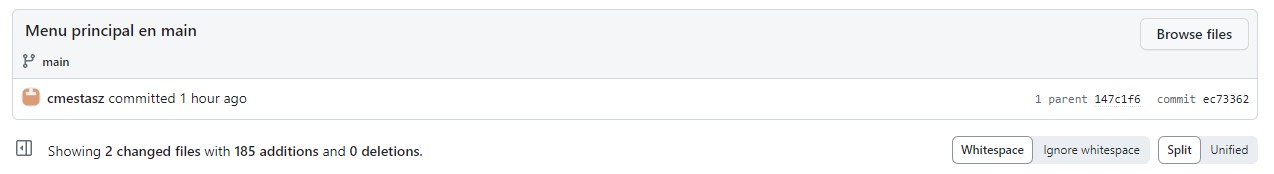
\includegraphics[width=1\textwidth,keepaspectratio]{img/commit01.jpg}
	\caption{Primer Commit.}
\end{figure}
\begin{figure}[H]
	\centering
	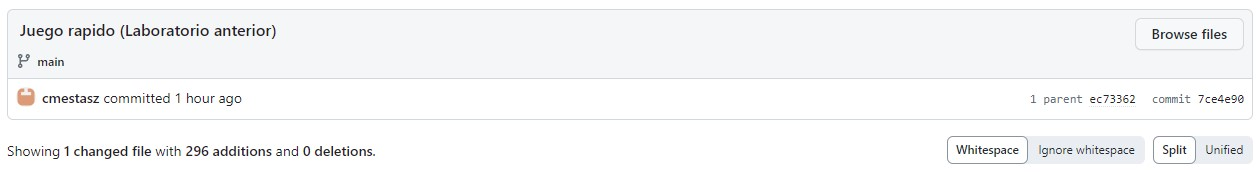
\includegraphics[width=1\textwidth,keepaspectratio]{img/commit02.jpg}
	\caption{Segundo Commit.}
\end{figure}
\begin{figure}[H]
	\centering
	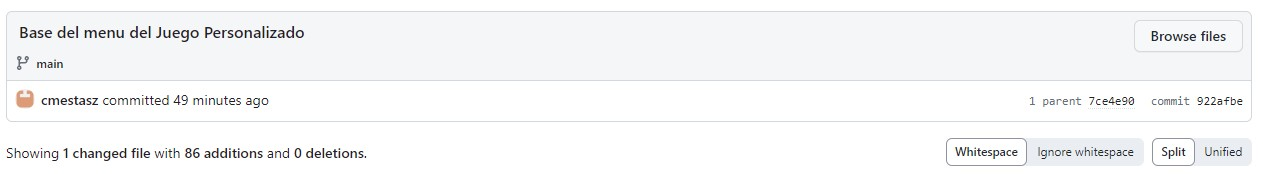
\includegraphics[width=1\textwidth,keepaspectratio]{img/commit03.jpg}
	\caption{Tercer Commit.}
\end{figure}
\begin{figure}[H]
	\centering
	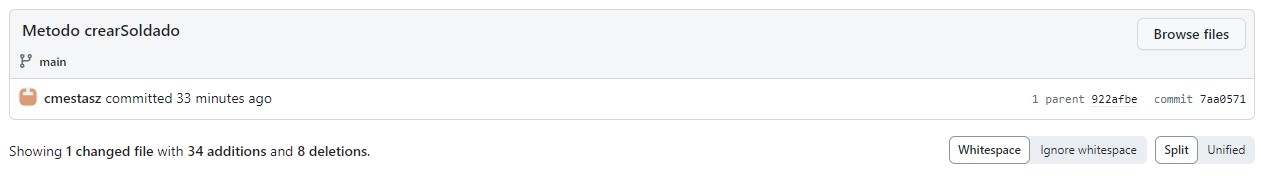
\includegraphics[width=1\textwidth,keepaspectratio]{img/commit04.jpg}
	\caption{Cuarto Commit.}
\end{figure}
\begin{figure}[H]
	\centering
	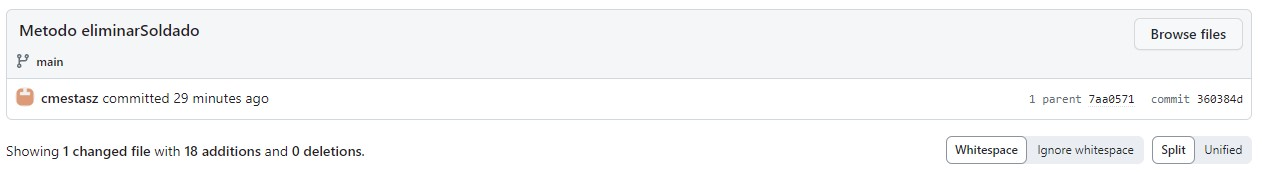
\includegraphics[width=1\textwidth,keepaspectratio]{img/commit05.jpg}
	\caption{Quinto Commit.}
\end{figure}
\begin{figure}[H]
	\centering
	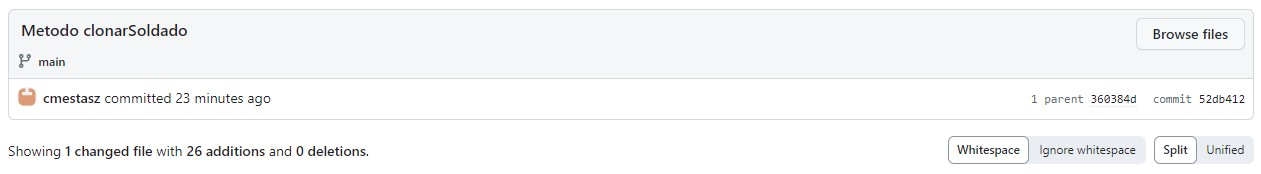
\includegraphics[width=1\textwidth,keepaspectratio]{img/commit06.jpg}
	\caption{Sexto Commit.}
\end{figure}
\begin{figure}[H]
	\centering
	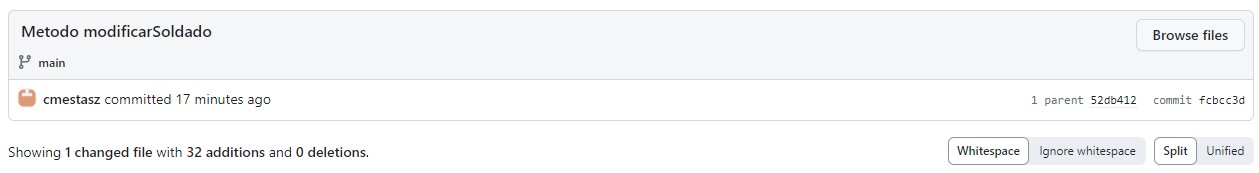
\includegraphics[width=1\textwidth,keepaspectratio]{img/commit07.jpg}
	\caption{Septimo Commit.}
\end{figure}
\begin{figure}[H]
	\centering
	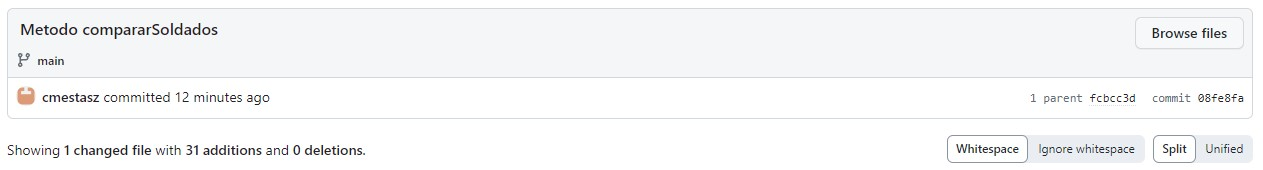
\includegraphics[width=1\textwidth,keepaspectratio]{img/commit08.jpg}
	\caption{Octavo Commit.}
\end{figure}
\begin{figure}[H]
	\centering
	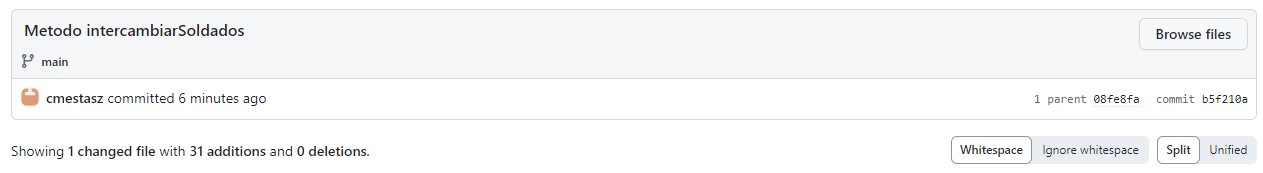
\includegraphics[width=1\textwidth,keepaspectratio]{img/commit09.jpg}
	\caption{Noveno Commit.}
\end{figure}
\begin{figure}[H]
	\centering
	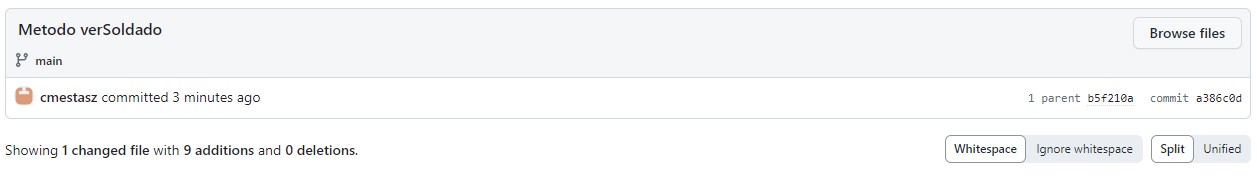
\includegraphics[width=1\textwidth,keepaspectratio]{img/commit10.jpg}
	\caption{Decimo Commit.}
\end{figure}
\begin{figure}[H]
	\centering
	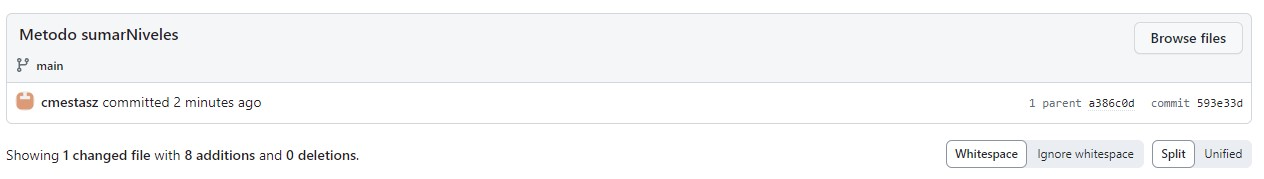
\includegraphics[width=1\textwidth,keepaspectratio]{img/commit11.jpg}
	\caption{Decimo Primer Commit.}
\end{figure}
\pagebreak

\section{Código desarrollado}
\lstinputlisting[language=Java, caption={Soldado.java},numbers=left,]{Soldado.java}
\begin{itemize}
	\item Clase que guarda nombre y vida del soldado.
	\item Posee tanto setters como getters para todos los atributos.
	\item Permite crear una copia con el metodo getCopia().
	\item Permite crear un nuevo soldado con la suma de los atributos de otros soldados con el metodo sumar().
	\item Posee el metodo toString() para poder imprimir el objeto.
\end{itemize}
\pagebreak
\lstinputlisting[language=Java, caption={VideoJuego5.java},numbers=left,]{VideoJuego9.java}
\begin{itemize}
	\item Método juegoRapido() contiene la batalla, para permitir el comportamiento iterativo.
	\item Método inicializarSoldados() crea a los soldados, los ubica en el tablero y los guarda en hashmaps de soldados por separado.
	\item Método imprimirTablero() imprime el tablero con ayuda de los métodos auxiliares generarEncabezado(), generarSeparacion() y generarFila(), ubicando a los soldados por su numero y ejercito.
	\item Método soldadoMayorVida() retorna el soldado con mayor vida de un ejército.
	\item Método promedioPuntosVida() retorna el promedio de los puntos de vida de todos los soldados de un ejército.
	\item Método imprimirSoldados() imprime los soldados del ejército.
	\item Método ordenarSoldadosBurbuja() ordena los soldados por vida de mayor a menor, usando ordenamiento burbuja.
	\item Método ordenarSoldadosSeleccion() ordena los soldados por vida de mayor a menor, usando ordenamiento selección.
	\item Se reusan los métodos para mostrar los datos de ambos ejércitos.
	\item Método juegoPersonalizado() contiene un menú que permite modificar el juego antes de iniciar.
	\item Método crearSoldado() permite crear un soldado.
	\item Método eliminarSoldado() permite eliminar un soldado.
	\item Método clonarSoldado() permite clonar un soldado y ponerlo en otra posición.
	\item Método modificarSoldado() permite modificar los atributos de un soldado.
	\item Método compararSoldados() permite comparar los atributos de dos soldados.
	\item Método intercambiarSoldados() permite intercambiar los atributos de dos soldados.
	\item Método verSoldado() permite mostrar un soldado por nombre.
	\item Método sumarNiveles() muestra la suma de atributos de todo el ejército.
	\item Método realizarCombates() se encarga de realizar el ciclo de juego, permitiendo a los jugadores seleccionar sus soldados, moverlos y atacar, hasta que quede un ganador.
\end{itemize}
\pagebreak

\section{Ejecución del código}
\lstinputlisting[keepspaces=true,language=bash,caption={VideoJuego9.java},numbers=left,]{ejec01.bash}
\pagebreak

\section{Estructura de laboratorio \itemPracticeNumber}
\begin{itemize}
	\item El contenido que se entrega en este laboratorio es el siguiente:
\end{itemize}
%%%%%%%%%%%%%%%%%%%%%%%%%%%%%%%%%%%%%%%%%%%%%%%%%%%%%%%%%%%%%%%%%%%%%%
\begin{lstlisting}[style=ascii-tree]
lab12/
|--- Soldado.java
|--- VideoJuego9.java
|--- commits.bash
|--- ejec01.bash
|--- Informe.tex
|--- Informe.pdf
|--- img
	|--- logo_abet.png
	|--- logo_episunsa.png
	|--- logo_unsa.jpg
	|--- commit01.jpg
	|--- commit02.jpg
	|--- commit03.jpg
	|--- commit04.jpg
	|--- commit05.jpg
	|--- commit06.jpg
	|--- commit07.jpg
	|--- commit08.jpg
	|--- commit09.jpg
	|--- commit10.jpg
	|--- commit11.jpg
\end{lstlisting}
%%%%%%%%%%%%%%%%%%%%%%%%%%%%%%%%%%%%%%%%%%%%%%%%%%%%%%%%%%%%%%%%%%%%%%
\pagebreak

\section{\textcolor{red}{Rúbricas}}

\subsection{\textcolor{red}{Entregable Informe}}
\begin{table}[H]
	\caption{Tipo de Informe}
	\setlength{\tabcolsep}{0.5em} % for the horizontal padding
	{\renewcommand{\arraystretch}{1.5}% for the vertical padding
		\begin{tabular}{|M{3cm}|M{12cm}|}
			\hline
			\multicolumn{2}{|c|}{\textbf{\textcolor{red}{Informe}}}                                                                                                      \\
			\hline
			\textbf{\textcolor{red}{Latex}} & \textcolor{blue}{El informe está en formato PDF desde Latex,  con un formato limpio (buena presentación) y facil de leer.} \\
			\hline
		\end{tabular}
	}
\end{table}

\subsection{\textcolor{red}{Rúbrica para el contenido del Informe y demostración}}
\begin{itemize}
	\item El alumno debe marcar o dejar en blanco en celdas de la columna \textbf{Checklist} si cumplio con el ítem correspondiente.
	\item Si un alumno supera la fecha de entrega, su calificación será sobre la nota mínima aprobatoria, siempre y cuando cumpla con todos los items.
	\item El alumno debe autocalificarse en la columna \textbf{Estudiante} de acuerdo a la siguiente tabla:

	      \begin{table}[ht]
		      \caption{Niveles de desempeño}
		      \begin{center}
			      \begin{tabular}{ccccc}
				      \hline
				                      & \multicolumn{4}{c}{Nivel}                                                              \\
				      \cline{1-5}
				      \textbf{Puntos} & Insatisfactorio 25\%      & En Proceso 50\% & Satisfactorio 75\% & Sobresaliente 100\% \\
				      \textbf{2.0}    & 0.5                       & 1.0             & 1.5                & 2.0                 \\
				      \textbf{4.0}    & 1.0                       & 2.0             & 3.0                & 4.0                 \\
				      \hline
			      \end{tabular}
		      \end{center}
	      \end{table}

\end{itemize}

\begin{table}[H]
	\caption{Rúbrica para contenido del Informe y demostración}
	\setlength{\tabcolsep}{0.5em} % for the horizontal padding
	{\renewcommand{\arraystretch}{1.5}% for the vertical padding
		%\begin{center}
		\begin{tabular}{|M{2.3cm}|M{5cm}|M{1.2cm}|M{1.5cm}|M{1.8cm}|M{1.4cm}|}
			\hline
			\multicolumn{2}{|c|}{Contenido y demostración} & Puntos                                                                                                                                                                                                        & Checklist & Estudiante & Profesor   \\
			\hline
			\textbf{1. GitHub}                             & Hay enlace URL activo del directorio para el laboratorio hacia su repositorio GitHub con código fuente terminado y fácil de revisar.                                                                          & 2         & X          & 2        & \\
			\hline
			\textbf{2. Commits}                            & Hay capturas de pantalla de los commits más importantes con sus explicaciones detalladas. (El profesor puede preguntar para refrendar calificación).                                                          & 4         & X          & 3        & \\
			\hline
			\textbf{3. Código fuente}                      & Hay porciones de código fuente importantes con numeración y explicaciones detalladas de sus funciones.                                                                                                        & 2         & X          & 2        & \\
			\hline
			\textbf{4. Ejecución}                          & Se incluyen ejecuciones/pruebas del código fuente explicadas gradualmente.                                                                                                                                    & 2         & X          & 1.5      & \\
			\hline
			\textbf{5. Pregunta}                           & Se responde con completitud a la pregunta formulada en la tarea. (El profesor puede preguntar para refrendar calificación).                                                                                   & 2         & X          & 2        & \\
			\hline
			\textbf{6. Fechas}                             & Las fechas de modificación del código fuente estan dentro de los plazos de fecha de entrega establecidos.                                                                                                     & 2         & X          & 2        & \\
			\hline
			\textbf{7. Ortografía}                         & El documento no muestra errores ortográficos.                                                                                                                                                                 & 2         & X          & 1.5      & \\
			\hline
			\textbf{8. Madurez}                            & El Informe muestra de manera general una evolución de la madurez del código fuente,  explicaciones puntuales pero precisas y un acabado impecable. (El profesor puede preguntar para refrendar calificación). & 4         & X          & 4        & \\
			\hline
			\multicolumn{2}{|c|}{\textbf{Total}}           & 20                                                                                                                                                                                                            &           & 18         &            \\
			\hline
		\end{tabular}
		%\end{center}
		%\label{tab:multicol}
	}
\end{table}

\section{Referencias}
\begin{itemize}
	\item Aedo, M. y Castro, E. (2021). FUNDAMENTOS DE PROGRAMACIÓN 2 - Tópicos de Programación Orientada a Objetos. Editorial UNSA.
\end{itemize}

%\pagebreak
%\bibliographystyle{apalike}
%\bibliographystyle{IEEEtranN}
%\bibliography{bibliography}

\end{document}